\documentclass[10pt,twocolumn]{article}
\usepackage{graphicx}
\usepackage[margin=0.75in,columnsep=0.3in]{geometry}
\usepackage{amsmath,amssymb}
\usepackage{booktabs}
\usepackage{hyperref}
\usepackage{float}
\usepackage{setspace}
\usepackage[font=small]{caption}
\usepackage{natbib}
\bibliographystyle{plainnat}

\hypersetup{colorlinks=true, linkcolor=black, urlcolor=blue, citecolor=black}
\singlespacing
\usepackage{abstract}
\usepackage{dblfloatfix}
\graphicspath{{../figures/}}

\title{\textbf{Can This Experiment Detect Anticipatory Utility?}\\
\large Identifiability and Power of a Delay-Manipulated Slot-Machine Task}

\author{Yonathan Amare}
\date{\today}

\begin{document}
\twocolumn[
\maketitle
\begin{onecolabstract}
\noindent
Anticipatory utility (AU) holds that people value not only a reward but the
experience of waiting for it. I designed a slot-machine task to test this
behaviourally: participants choose between a sure amount (SAFE) and an
equal-expected-value gamble (BET), and after a winning BET the payout arrives
after a machine-specific delay of 8, 12 or 16 seconds. If savouring is real,
longer delays should make BET more attractive even though the money is
identical. Before collecting data, I ask whether this design can detect the
effect at all.

Using simulated participants drawn from a reinforcement-learning model with
and without an anticipatory term, I run parameter recovery, model recovery and
a power analysis of the planned test. The original design is underpowered.
With the planned pilot of 30 participants and a moderate savouring effect, the
planned regression detects AU in 43\% of simulated studies. Per-participant
model comparison classifies a true savourer as AU only 42\% of the time under
AIC and 23\% under BIC, and a quarter of fitted inverse temperatures hit their
upper bound. A redesign that widens the delays to 2, 9 and 16 seconds and
raises trials from 12 to 30 per machine reaches 95\% power with the same 30
participants. No human data are used; the contribution is a design check that
should precede data collection.
\end{onecolabstract}
\vspace{1em}
]


\section{Introduction}

\citet{loewenstein1987} proposed that the value of a delayed outcome includes
the utility of anticipating it, which can make people prefer to delay pleasant
outcomes. \citet{iigaya2016} formalised savouring in a reinforcement-learning
framework and showed that anticipation is boosted by the prediction error
generated by an informative cue. Behaviourally isolating anticipatory utility is
hard, because delay, probability and magnitude usually change together.

The task studied here holds expected value fixed and manipulates only the
delay between a win cue and payment. I built it in Gorilla during a 2025
mentored MA research project at the Iigaya Lab; data collection did not take
place before the project ended. This paper asks the question that should come
first: \emph{if anticipatory utility exists at a plausible strength, would the
planned study detect it?} Following the recommendations of
\citet{wilson2019}, I answer it by simulating participants with known
parameters and checking whether the planned analyses recover them.

\section{The task}

Each trial offers SAFE, a sure amount paid immediately, or BET, which pays
twice that amount with probability $0.5$ and nothing otherwise, so the two have
equal expected value. A winning BET shows a win cue, then pays after the
delay assigned to its machine: $8$\,s for machine A, $12$\,s for B and $16$\,s
for C. A losing BET pays nothing immediately. The task has 36 main trials,
12 per machine, with stakes between \$4 and \$11. Two catch trials offer
SAFE \$25 against a \$20 BET, where SAFE clearly dominates, to check attention.
Trial order is randomised per participant. The full trial list is the Gorilla
spreadsheet in the accompanying repository.

\section{Models}

Both models learn each machine's win probability from the outcomes of BET
choices,
\begin{equation}
\hat p_m \leftarrow \hat p_m + \alpha\,(o_t - \hat p_m), \qquad \hat p_m^{(0)} = 0.5,
\end{equation}
updated only after a BET on machine $m$, and choose with a logistic rule,
\begin{equation}
P(\text{BET}_t) = \sigma\!\left(\beta\,[\,Q_{\text{bet},t} - Q_{\text{safe},t}\,]\right),
\qquad Q_{\text{safe},t} = S_t,
\end{equation}
with amounts in units of \$10.

\paragraph{EV-RL.} The value of betting is its learned expected value plus a
general taste for gambling,
\begin{equation}
Q_{\text{bet},t} = \hat p_m H_t + b,
\end{equation}
where $H_t$ is the winning amount. Parameters are $(\alpha, \beta, b)$.

\paragraph{AU-RL.} A win is worth more when it can be savoured for longer,
\begin{equation}
Q_{\text{bet},t} = \hat p_m H_t \left(1 + \kappa\,\frac{D_m}{16\text{ s}}\right) + b,
\end{equation}
where $D_m$ is the machine's delay. The parameter $\kappa$ is the extra value of
a win, as a fraction of the prize, at the longest delay; $\kappa > 0$ is
savouring and $\kappa < 0$ dread. The bias $b$ shifts BET equally on every
machine, so only $\kappa$ can produce a preference that changes with delay.
This is what makes the two models separable in principle.

\section{Methods}

\paragraph{Simulated participants.} Each simulated participant draws
$\alpha \sim U(0.05, 0.6)$, $\beta \sim U(1, 8)$ and $b \sim N(0, 0.3^2)$; AU
participants also draw $\kappa$. These ranges are assumptions chosen to give
choice behaviour that is neither deterministic nor random, not estimates from
real data.

\paragraph{Fitting.} Both models are fitted per participant by maximum
likelihood with L-BFGS-B under box constraints, from five random starting
points, keeping the best. Models are compared with AIC and BIC.

\paragraph{Analyses.} (i) \emph{Parameter recovery:} 200 AU participants with
$\kappa \sim U(0,1)$, fitted with AU-RL. (ii) \emph{Model recovery:} 100
participants from each model, with $\kappa \sim U(0.3, 1)$ for AU, each fitted
with both models. (iii) \emph{Power:} for $N \in \{15, 30, 60, 120\}$ and
$\kappa \in \{0, 0.25, 0.5, 1\}$, 150 simulated studies per cell, each analysed
with the planned test: a logistic regression of BET on delay over the
EV-matched trials, with standard errors clustered by participant (GEE,
exchangeable working correlation), one-sided at $\alpha = 0.05$. The planned
regression also included $\operatorname{logit}(p)$, but every BET in the final
design has $p = 0.5$, so that term is constant and drops out.

\paragraph{Redesign.} Each analysis is repeated for a proposed design with
delays of 2, 9 and 16\,s and 30 EV-matched trials per machine (92 trials in
total including the two catch trials), keeping the original stake levels.

\section{Results}

\subsection{Parameter recovery}

\begin{figure*}[t]
\centering
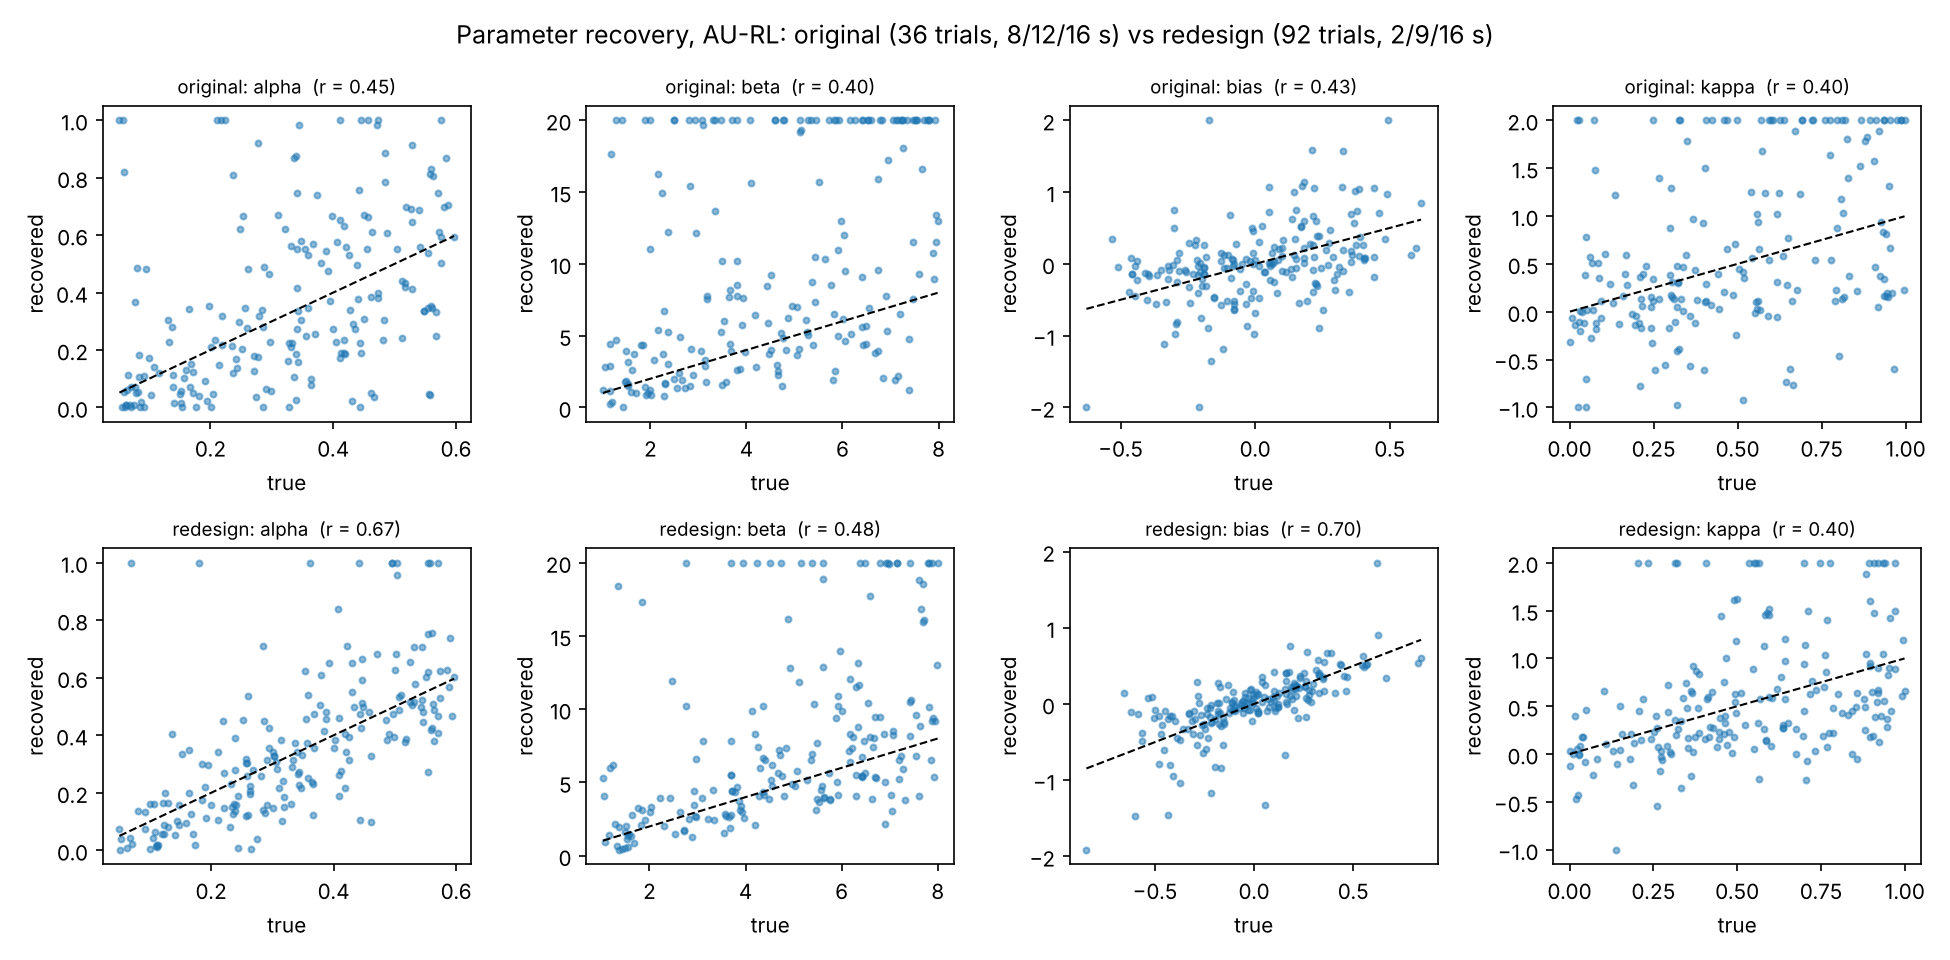
\includegraphics[width=\textwidth]{parameter_recovery.png}
\caption{True against recovered parameters for 200 simulated AU participants.
Top row: original design. Bottom row: redesign.}
\label{fig:recovery}
\end{figure*}

\begin{table}[t]
\centering
\small
\caption{Parameter recovery. Rank correlation between true and recovered
values, and the share of fits stuck at a bound.}
\label{tab:recovery}
\setlength{\tabcolsep}{3pt}
\begin{tabular}{lcccc}
\toprule
& \multicolumn{2}{c}{Original} & \multicolumn{2}{c}{Redesign} \\
\cmidrule(lr){2-3} \cmidrule(lr){4-5}
Parameter & Rank corr. & At bound & Rank corr. & At bound \\
\midrule
$\alpha$ & 0.51 & 10\% & 0.74 & 5\% \\
$\beta$  & 0.46 & 27\% & 0.60 & 11\% \\
$b$      & 0.44 & 2\%  & 0.77 & 0\% \\
$\kappa$ & 0.42 & 19\% & 0.48 & 10\% \\
\bottomrule
\end{tabular}
\end{table}

With 36 trials per participant, recovery is weak for every parameter
(Table~\ref{tab:recovery}, Figure~\ref{fig:recovery}). A quarter of the
inverse-temperature estimates run to the upper bound, which happens when a
participant's choices are nearly all one option. The redesign improves
$\alpha$, $\beta$ and $b$ substantially and halves the share of $\kappa$ fits at
a bound, but individual $\kappa$ estimates remain noisy in both designs.
Individual-level $\kappa$ should not be interpreted on its own.

\subsection{Model recovery}

\begin{table}[t]
\centering
\small
\caption{Share of simulated participants for which each criterion selects the
true model.}
\label{tab:modelrec}
\begin{tabular}{lcccc}
\toprule
& \multicolumn{2}{c}{Original} & \multicolumn{2}{c}{Redesign} \\
\cmidrule(lr){2-3} \cmidrule(lr){4-5}
True model & AIC & BIC & AIC & BIC \\
\midrule
EV-RL & 80\% & 93\% & 83\% & 96\% \\
AU-RL ($\kappa \in [0.3, 1]$) & 42\% & 23\% & 66\% & 50\% \\
\bottomrule
\end{tabular}
\end{table}

Under the original design, a participant who genuinely savours is classified as
AU only 42\% of the time by AIC and 23\% by BIC
(Table~\ref{tab:modelrec}). The planned per-participant comparison would lean
towards ``no anticipatory utility'' even when it is present. The redesign
improves sensitivity to 66\% under AIC while keeping specificity above 80\%.

\subsection{Power}

\begin{figure*}[t]
\centering
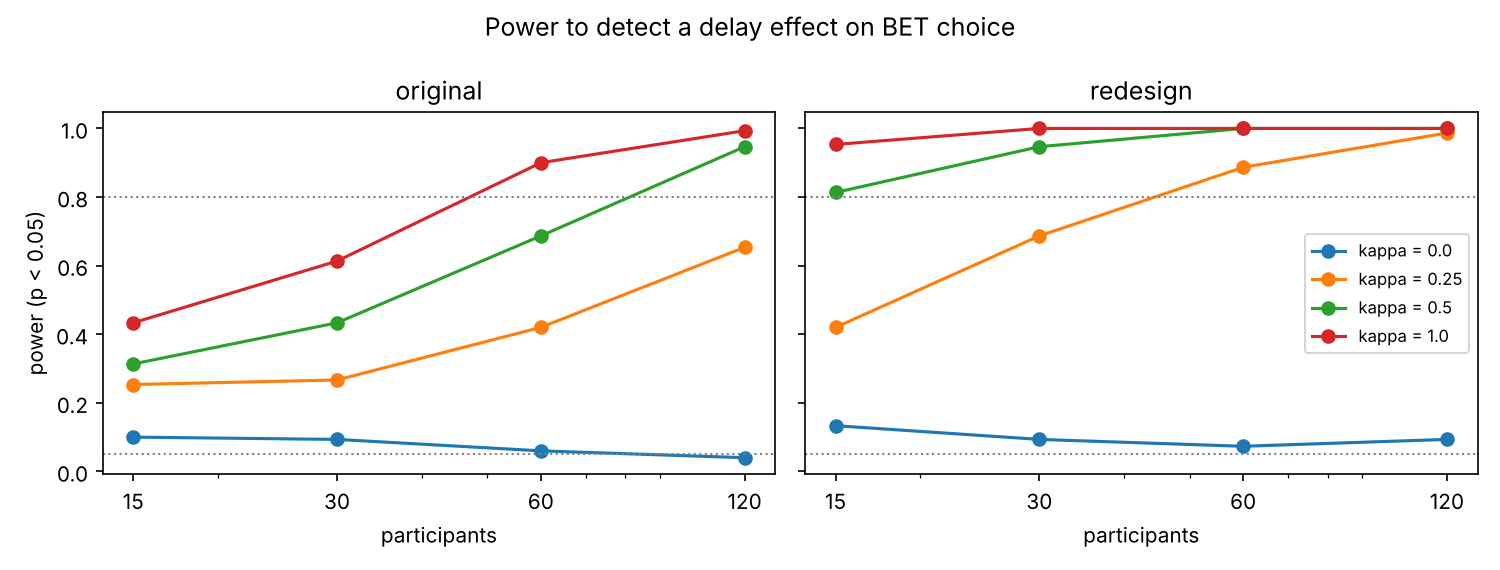
\includegraphics[width=0.85\textwidth]{power.png}
\caption{Power of the planned delay test by sample size and true $\kappa$.
Dotted lines mark 5\% and 80\%.}
\label{fig:power}
\end{figure*}

\begin{table}[t]
\centering
\small
\caption{Share of 150 simulated studies with a significant positive delay
effect ($p < 0.05$, one-sided). Rows with $\kappa = 0$ are false-positive
rates.}
\label{tab:power}
\setlength{\tabcolsep}{4pt}
\begin{tabular}{llcccc}
\toprule
Design & $\kappa$ & $N=15$ & $N=30$ & $N=60$ & $N=120$ \\
\midrule
Original & 0    & 0.10 & 0.09 & 0.06 & 0.04 \\
         & 0.25 & 0.25 & 0.27 & 0.42 & 0.65 \\
         & 0.5  & 0.31 & \textbf{0.43} & 0.69 & 0.95 \\
         & 1.0  & 0.43 & 0.61 & 0.90 & 0.99 \\
\midrule
Redesign & 0    & 0.13 & 0.09 & 0.07 & 0.09 \\
         & 0.25 & 0.42 & 0.69 & 0.89 & 0.99 \\
         & 0.5  & 0.81 & \textbf{0.95} & 1.00 & 1.00 \\
         & 1.0  & 0.95 & 1.00 & 1.00 & 1.00 \\
\bottomrule
\end{tabular}
\end{table}

With the planned pilot of 30 participants and $\kappa = 0.5$, the original
design detects the effect in 43\% of simulated studies
(Table~\ref{tab:power}, Figure~\ref{fig:power}). Reaching 80\% power would take
roughly 60 to 120 participants. The redesign reaches 95\% with 30 participants
and still detects a weaker effect ($\kappa = 0.25$) in 69\% of studies.

A single simulated pilot can look far better than the design deserves. One draw
of 30 participants at $\kappa = 0.5$ under the original design gave a highly
significant slope, while the same design fails in most draws. Power, not one
sample, is the right basis for judging a design.

\section{Discussion}

\paragraph{Why the original design struggles.} Two features limit it. First,
the delays are close together: at 8, 12 and 16\,s the savouring term only
doubles from the shortest to the longest machine, so a given $\kappa$ moves
choices little. Spreading the delays to 2, 9 and 16\,s gives an eightfold
range. Second, 12 choices per machine leave each participant's choice rate very
noisy; 30 per machine reduce that noise substantially.

\paragraph{Recommended analysis.} Per-participant model selection under-detects
AU at realistic trial counts. The primary test should be group-level: the
clustered or mixed-effects regression of choice on delay used here, or a
hierarchical fit of $\kappa$ that pools information across participants.

\paragraph{Limitations.}
\begin{itemize}
\item The false-positive rate is somewhat above 5\% (9--13\%) at small $N$ and
in the redesign, consistent with the known small-sample bias of GEE sandwich
standard errors. A permutation test or bias-corrected sandwich estimator would
correct this in a real study.
\item Savouring is modelled as linear in delay. If it saturates, as in
\citet{iigaya2016}, a wide delay range matters even more.
\item True win probabilities equal the prior of 0.5, so the learning rate is
only weakly identified by design. This is acceptable for testing AU but limits
what the task can say about learning.
\item The simulated parameter ranges are assumptions. Pilot data would allow
them to be calibrated.
\item The prediction-error boost to savouring proposed by \citet{iigaya2016} is
not identifiable here, because every BET has the same win probability. Testing
it requires machines that differ in win probability as well as delay, crossed
so that the two do not move together.
\end{itemize}

\section{Conclusion}

As built, the task is unlikely to detect a moderate anticipatory-utility effect
in a 30-person pilot, and per-participant model comparison would mostly miss it.
Widening the delay range and increasing trials per machine raises power from
43\% to 95\% at the same sample size. Simulating the planned analysis before
collecting data turns an underpowered pilot into an informative one.

\section*{Reproducibility}

Code, the task spreadsheet and all results:
\url{https://github.com/yamare1/anticipatory-utility-power}. All results
regenerate from four scripts with fixed random seeds.

\bibliography{refs}

\end{document}
